Swanson initially identified three categories of software changes: corrective, adaptive, and perfective~\cite{Swanson1976:Dimension}. These categories were updated later and ISO/IEC 14764 instead presents four types of changes: corrective, adaptive, perfective, and preventive~\cite{iso}.

\subsection{Corrective Change} 
Corrective change refers software modifications initiated by software defects. A defect can result from design errors, logic errors, and coding errors~\cite{Longstreet1990:smc}.

\begin{itemize}
\item Design errors: software design does not fully align with the requirements specification. The faulty design leads to a software system that either incompletely or incorrectly implements the requested computational functionality. 
\item Logic errors: a program behaves abnormally by terminating unexpectedly or producing wrong outputs. The abnormal behaviors are mainly due to flaws in software functionality implementations.
\item Coding errors: although a program can function well, it takes excessively high runtime or memory overhead before responding to user requests. Such failures may be caused by loose coding, or the absence of {\em reasonableness checks} on computations performed.
\end{itemize}

\subsection{Adaptive Change}
Adaptive change is a change introduced to accommodate any modifications in the environment of a software product. The term \textbf{environment} here refers to the totality of all conditions that influence the software product, including business rules, government policies, and software and hardware operating systems. For example, when a library or platform developers may evolve its APIs, the corresponding adaptation may be required for client applications to handle such environment change. As another example, when porting a mobile application from Android to iOS, mobile developers need to apply adaptive changes to translate the code from Java to Swift, so that the software is still compilable and executable on the new platform.  
%when maintaining a legacy system that was written in Fortran decades ago, programmers may migrate the system to a mainstream general purpose language, such as Java, to facilitate the maintenance of existing codebase and to extend the system by leveraging new features of the popular language. When building phone apps, Mobile developers may port a mobile application from one platform (e.g., Android) to another (e.g. iOS) by translating code from Java to Swift. 
\subsection{Perfective Change}

Perfective change is the change undertaken to expand the existing requirements of a system~\cite{Seaman2008:SMC}. When a software product becomes useful, users always expect to use it in new scenarios beyond the scope for which it was initially developed. Such requirement expansion causes changes to either enhance existing system functionality or to add new features. For instance, an image processing system is originally developed to process JPEG files, and later goes through a series of perfective changes to handle other formats of images, such as PNG and SVG. The nature and characteristics of new feature addition is not necessarily easy to define and in fact understudied for that reason. In Section~\ref{sec:perfective}, we discuss a rather well-understood type of perfective changes, called {\em crosscutting concerns} and then present tool and language support for adding crosscutting concerns. Crosscutting concerns refer to the {\em secondary design decisions} such as logging, performance, error handling, and synchronization. Adding these secondary concerns often involves non-localized changes throughout the system, due to the {\em tyranny} of dominant design decisions already implemented in the system. Concerns that are added later may end up being scattered across many modules and thus tangled with one another. 

\subsection{Preventive Change}
Preventive change is the change applied to prevent malfunctions or to improve maintainability of software. 
According to Lehman's laws of software evolution~\cite{Lehman1984:ULE}, the long-term effect of corrective, adaptive, and perfective changes is deteriorating the software structure, while increasing entropy. Preventive changes are usually applied to address the problems. For instance, after developers fix some bugs and implement new features in an existing software product, the complexity of source code can increase to an unmanageable level. Through code refactoring---a series of behavior-preserving changes, developers can reduce the code complexity, and increase the readability, reusability, and maintainability of software.
\begin{figure}[!htb]
\centering
\scalebox{0.5}{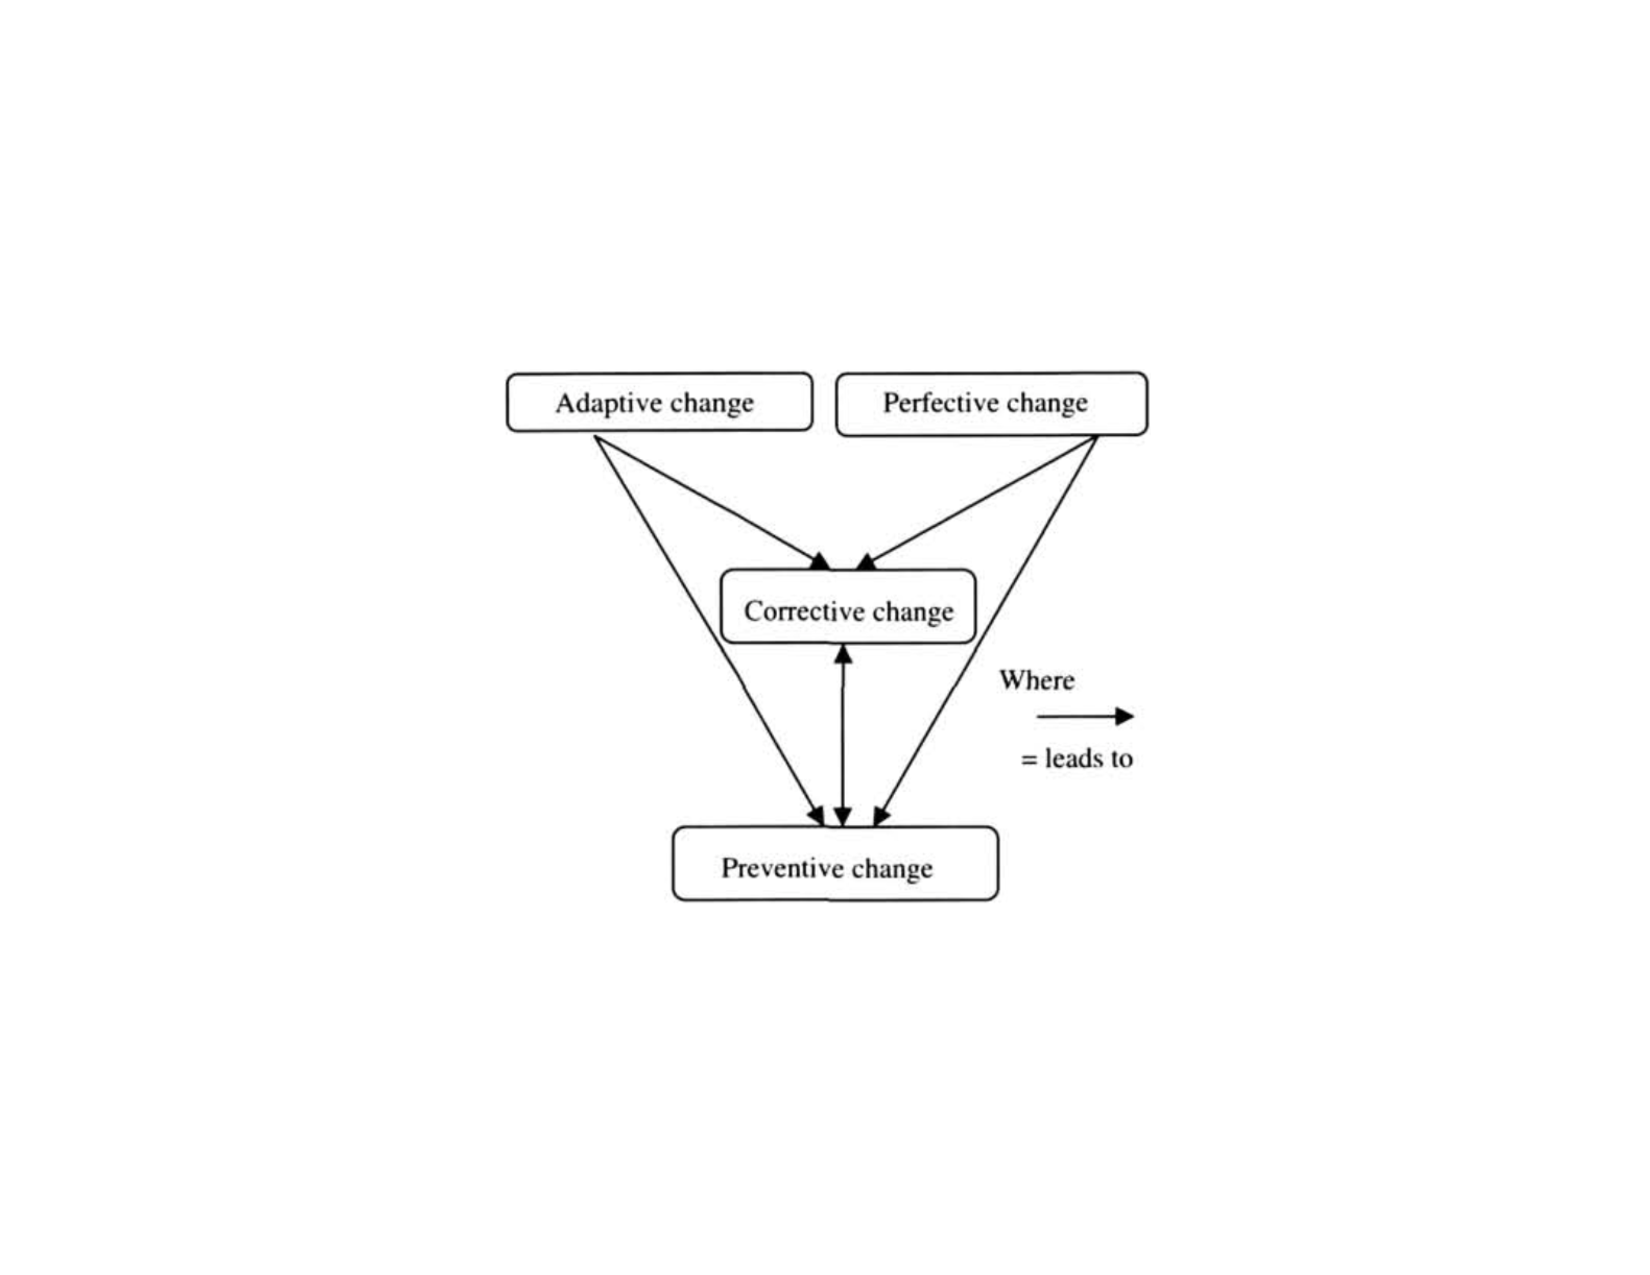
\includegraphics{images/relationship_of_changes.pdf}}
\caption{Potential relation between software changes~\cite{Seaman2008:SMC}}
\label{fig:relation}
\end{figure}

Figure~\ref{fig:relation} presents the potential relationships between different types of changes~\cite{Seaman2008:SMC}. Specifically, both adaptive changes and perfective changes may lead to the other two types of changes, because developers may introduce bugs or worsen code structures when adapting software to new environments or implementing new features.

